\clearpage

\section*{Přizpůsobený filtr}

\begin{figure}[H]
    \centering
    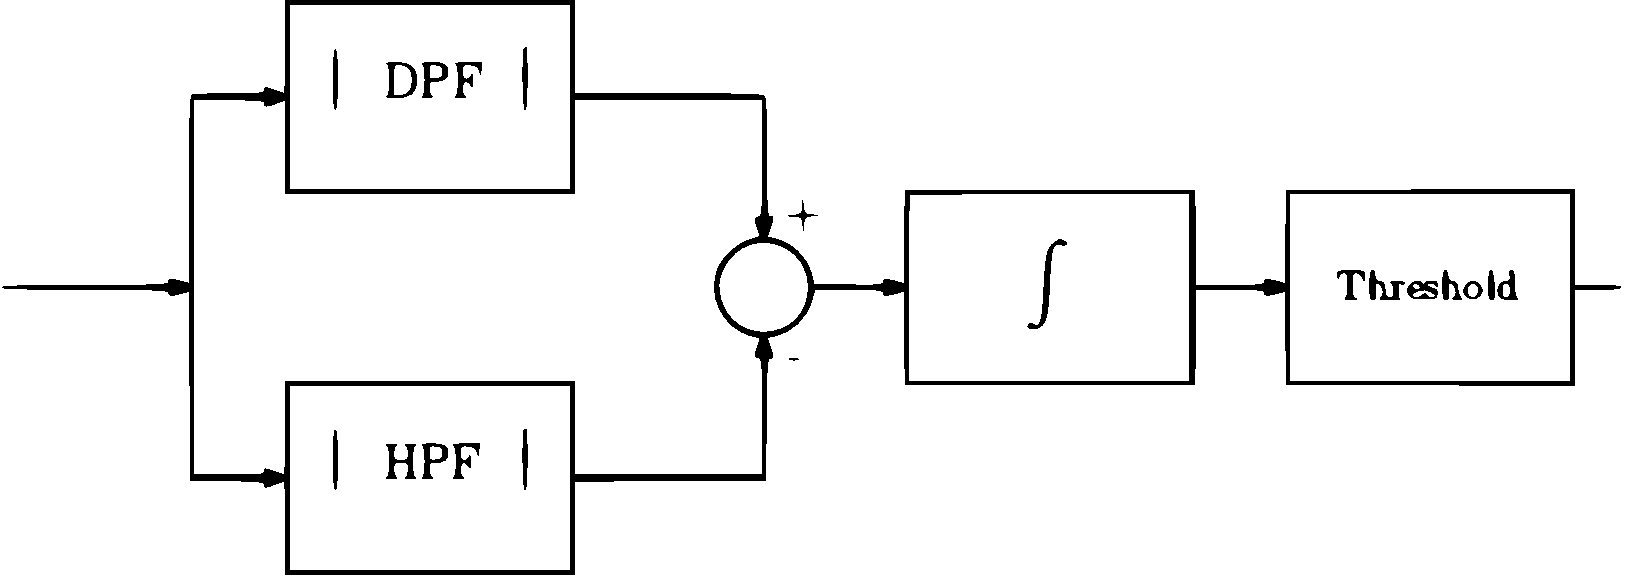
\includegraphics[width=0.5\textwidth]{img/dem1.pdf}
    \caption{Blokové schéma demodulátoru s přizpůsobeným filtrem}
\end{figure}

Tato metoda bude dále označována jako DEM1. Nejprve dojde k rozdělení signálu pomocí horní a dolní propusti. Následně je spočítána absolutní hodnota z filtrovaných signálů, což představuje usměrnění. Díky tomu je možné signály od sebe odečíst. Tím vznikne signál ve kterém vyšším hodnotám odpovídá 1 nízkým 0. Poté signál integrujeme podle času, tedy opět na něj aplikujeme dolní propust. Nyní je signál již připraven k prahování, pomocí kterého rozhodneme zda-li je přijímána logická nula nebo jednička.

\begin{figure}[H]
    \centering
    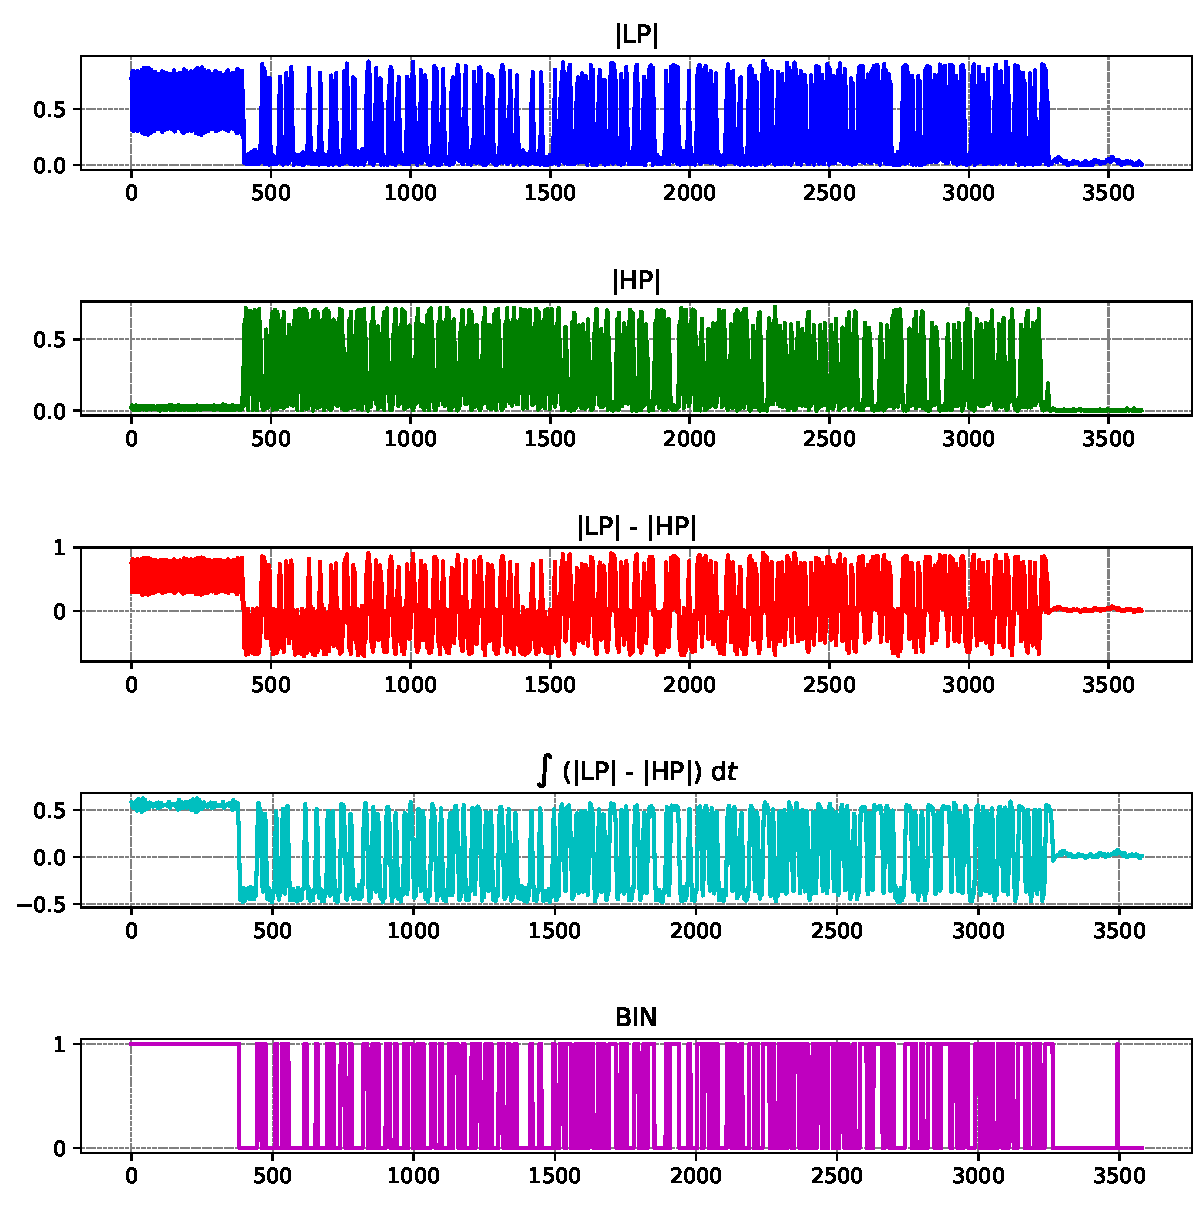
\includegraphics[width=0.85\textwidth]{img/dem1_graph.pdf}
    \caption{Časové průběhy bloků demodulátoru}
\end{figure}